\documentclass[10,portrait]{article}
\usepackage{lmodern}
\usepackage{amssymb,amsmath}
\usepackage{ifxetex,ifluatex}
\usepackage{fixltx2e} % provides \textsubscript
\ifnum 0\ifxetex 1\fi\ifluatex 1\fi=0 % if pdftex
  \usepackage[T1]{fontenc}
  \usepackage[utf8]{inputenc}
\else % if luatex or xelatex
  \ifxetex
    \usepackage{mathspec}
  \else
    \usepackage{fontspec}
  \fi
  \defaultfontfeatures{Ligatures=TeX,Scale=MatchLowercase}
\fi
% use upquote if available, for straight quotes in verbatim environments
\IfFileExists{upquote.sty}{\usepackage{upquote}}{}
% use microtype if available
\IfFileExists{microtype.sty}{%
\usepackage[]{microtype}
\UseMicrotypeSet[protrusion]{basicmath} % disable protrusion for tt fonts
}{}
\PassOptionsToPackage{hyphens}{url} % url is loaded by hyperref
\usepackage[unicode=true]{hyperref}
\PassOptionsToPackage{usenames,dvipsnames}{color} % color is loaded by hyperref
\hypersetup{
            pdftitle={Using git and Github for research and life},
            colorlinks=true,
            linkcolor=blue,
            citecolor=red,
            urlcolor=blue,
            breaklinks=true}
\urlstyle{same}  % don't use monospace font for urls
\usepackage[margin=1in]{geometry}
\usepackage[]{biblatex}
\usepackage{color}
\usepackage{fancyvrb}
\newcommand{\VerbBar}{|}
\newcommand{\VERB}{\Verb[commandchars=\\\{\}]}
\DefineVerbatimEnvironment{Highlighting}{Verbatim}{commandchars=\\\{\}}
% Add ',fontsize=\small' for more characters per line
\usepackage{framed}
\definecolor{shadecolor}{RGB}{248,248,248}
\newenvironment{Shaded}{\begin{snugshade}}{\end{snugshade}}
\newcommand{\KeywordTok}[1]{\textcolor[rgb]{0.13,0.29,0.53}{\textbf{#1}}}
\newcommand{\DataTypeTok}[1]{\textcolor[rgb]{0.13,0.29,0.53}{#1}}
\newcommand{\DecValTok}[1]{\textcolor[rgb]{0.00,0.00,0.81}{#1}}
\newcommand{\BaseNTok}[1]{\textcolor[rgb]{0.00,0.00,0.81}{#1}}
\newcommand{\FloatTok}[1]{\textcolor[rgb]{0.00,0.00,0.81}{#1}}
\newcommand{\ConstantTok}[1]{\textcolor[rgb]{0.00,0.00,0.00}{#1}}
\newcommand{\CharTok}[1]{\textcolor[rgb]{0.31,0.60,0.02}{#1}}
\newcommand{\SpecialCharTok}[1]{\textcolor[rgb]{0.00,0.00,0.00}{#1}}
\newcommand{\StringTok}[1]{\textcolor[rgb]{0.31,0.60,0.02}{#1}}
\newcommand{\VerbatimStringTok}[1]{\textcolor[rgb]{0.31,0.60,0.02}{#1}}
\newcommand{\SpecialStringTok}[1]{\textcolor[rgb]{0.31,0.60,0.02}{#1}}
\newcommand{\ImportTok}[1]{#1}
\newcommand{\CommentTok}[1]{\textcolor[rgb]{0.56,0.35,0.01}{\textit{#1}}}
\newcommand{\DocumentationTok}[1]{\textcolor[rgb]{0.56,0.35,0.01}{\textbf{\textit{#1}}}}
\newcommand{\AnnotationTok}[1]{\textcolor[rgb]{0.56,0.35,0.01}{\textbf{\textit{#1}}}}
\newcommand{\CommentVarTok}[1]{\textcolor[rgb]{0.56,0.35,0.01}{\textbf{\textit{#1}}}}
\newcommand{\OtherTok}[1]{\textcolor[rgb]{0.56,0.35,0.01}{#1}}
\newcommand{\FunctionTok}[1]{\textcolor[rgb]{0.00,0.00,0.00}{#1}}
\newcommand{\VariableTok}[1]{\textcolor[rgb]{0.00,0.00,0.00}{#1}}
\newcommand{\ControlFlowTok}[1]{\textcolor[rgb]{0.13,0.29,0.53}{\textbf{#1}}}
\newcommand{\OperatorTok}[1]{\textcolor[rgb]{0.81,0.36,0.00}{\textbf{#1}}}
\newcommand{\BuiltInTok}[1]{#1}
\newcommand{\ExtensionTok}[1]{#1}
\newcommand{\PreprocessorTok}[1]{\textcolor[rgb]{0.56,0.35,0.01}{\textit{#1}}}
\newcommand{\AttributeTok}[1]{\textcolor[rgb]{0.77,0.63,0.00}{#1}}
\newcommand{\RegionMarkerTok}[1]{#1}
\newcommand{\InformationTok}[1]{\textcolor[rgb]{0.56,0.35,0.01}{\textbf{\textit{#1}}}}
\newcommand{\WarningTok}[1]{\textcolor[rgb]{0.56,0.35,0.01}{\textbf{\textit{#1}}}}
\newcommand{\AlertTok}[1]{\textcolor[rgb]{0.94,0.16,0.16}{#1}}
\newcommand{\ErrorTok}[1]{\textcolor[rgb]{0.64,0.00,0.00}{\textbf{#1}}}
\newcommand{\NormalTok}[1]{#1}
\usepackage{graphicx,grffile}
\makeatletter
\def\maxwidth{\ifdim\Gin@nat@width>\linewidth\linewidth\else\Gin@nat@width\fi}
\def\maxheight{\ifdim\Gin@nat@height>\textheight\textheight\else\Gin@nat@height\fi}
\makeatother
% Scale images if necessary, so that they will not overflow the page
% margins by default, and it is still possible to overwrite the defaults
% using explicit options in \includegraphics[width, height, ...]{}
\setkeys{Gin}{width=\maxwidth,height=\maxheight,keepaspectratio}
\IfFileExists{parskip.sty}{%
\usepackage{parskip}
}{% else
\setlength{\parindent}{0pt}
\setlength{\parskip}{6pt plus 2pt minus 1pt}
}
\setlength{\emergencystretch}{3em}  % prevent overfull lines
\providecommand{\tightlist}{%
  \setlength{\itemsep}{0pt}\setlength{\parskip}{0pt}}
\setcounter{secnumdepth}{0}
% Redefines (sub)paragraphs to behave more like sections
\ifx\paragraph\undefined\else
\let\oldparagraph\paragraph
\renewcommand{\paragraph}[1]{\oldparagraph{#1}\mbox{}}
\fi
\ifx\subparagraph\undefined\else
\let\oldsubparagraph\subparagraph
\renewcommand{\subparagraph}[1]{\oldsubparagraph{#1}\mbox{}}
\fi

% set default figure placement to htbp
\makeatletter
\def\fps@figure{htbp}
\makeatother


\title{Using git and Github for research and life}
\author{Matthew
Malishev\textsuperscript{1}*\\[2\baselineskip]\emph{\textsuperscript{1}
Department of Biology, Emory University, 1510 Clifton Road NE, Atlanta,
GA, USA, 30322}}
\date{}

\begin{document}
\maketitle

{
\hypersetup{linkcolor=black}
\setcounter{tocdepth}{3}
\tableofcontents
}
\newpage   

Date: 2019-03-11\\
R version: 3.5.0\\
*Corresponding author:
\href{mailto:matthew.malishev@gmail.com}{\nolinkurl{matthew.malishev@gmail.com}}\\
This document can be found at
\url{https://github.com/darwinanddavis/githubpres}

\newpage    

\subsection{1. Install git}\label{install-git}

\emph{Mac users}\\
\href{https://git-scm.com/book/en/v2/Getting-Started-Installing-Git}{Install
git}.

\emph{Windows users}\\
\href{https://www.sitereq.com/post/easiest-way-to-install-git-bash-commands-on-windows\#git-bash-windows-installation}{Install
git with Git Bash}. Git Bash is a text editor for running git commands.

~ ~ ~

\textbf{Once installed, confirm git is on your computer}

\emph{Mac}

Go to \emph{Applications} \textgreater{} \emph{Utilities} \textgreater{}
\emph{Terminal}. In Terminal, type the following and press Enter:

\begin{Shaded}
\begin{Highlighting}[]

\FunctionTok{git}\NormalTok{ --version }
\end{Highlighting}
\end{Shaded}

If you don't see anything like \texttt{git\ version\ 2.10.0}, try the
reinstallation steps again. Close the Terminal.

\emph{Windows}

Open Git Bash and type in the following and press Enter:

\begin{Shaded}
\begin{Highlighting}[]

\FunctionTok{git}\NormalTok{ --version  }
\end{Highlighting}
\end{Shaded}

If you don't see anything like \texttt{git\ version\ 2.20.1.windows.1},
try the reinstallation steps again. Close Git Bash.

~ ~ ~

\textbf{If you can't get it working, email me before the workshop and
I'll help you.}

\newpage  

\subsection{2. Configure your user name and
email}\label{configure-your-user-name-and-email}

Once \texttt{git} is installed, you then just need to configure your
user credentials.

Using either Terminal for Mac or Git Bash for Windows, type the
following and press Enter:

\begin{Shaded}
\begin{Highlighting}[]

\FunctionTok{git}\NormalTok{ config --global user.name }\StringTok{"Your Name"} 
\end{Highlighting}
\end{Shaded}

Then type this to configure your email and press Enter:

\begin{Shaded}
\begin{Highlighting}[]

\FunctionTok{git}\NormalTok{ config --global user.email }\StringTok{"your@email.com"} 
\end{Highlighting}
\end{Shaded}

~ ~ ~

\paragraph{You're set!}\label{youre-set}

Once \texttt{git} is on your computer, you can now access its features
using your local computer for version control.

\newpage  

\subsection{3. Create a Github account}\label{create-a-github-account}

Create your Github account so you can push your documents to the cloud.

\href{https://github.com/}{Create your new Github account}. Some tips on
creating an account:

\begin{itemize}
\tightlist
\item
  Choose a username that you plan to keep. Something that represents
  your professional acumen, e.g.~not ``matt\_loves\_hiphop86''\\
  \hspace*{0.333em}
\item
  Github is universal and really useful. You can connect to programming,
  troubleshooting, userX sites, and coding libraries, e.g.~CodePen,
  using your Github account, so plan for longevity.\\
  \hspace*{0.333em}
\end{itemize}

Feel free to navigate my personal Github page. Everything is publicly
available.

\url{www.github.com/darwinanddavis}

Some essential elements of your Github page:

\begin{itemize}
\tightlist
\item
  Your repositories. This is where you store your online information.\\
  \hspace*{0.333em}
\item
  Your gits. These are the digital footprints of your changes. We use
  this for
  \href{https://git-scm.com/book/en/v2/Getting-Started-About-Version-Control}{version
  control}.\\
  \hspace*{0.333em}
\item
  Your README.md file. This tells users what your repo contains,
  instructions for running code, troubleshooting, version control, links
  to external web sources, and other git specific elements, such as
  program/package versions.\\
  \hspace*{0.333em}
\end{itemize}

\begin{center}\rule{0.5\linewidth}{\linethickness}\end{center}

~ ~ \textbf{End installation instructions.} The following sections
contain reference guides for your Github page and using git and bash
commands (talking to git). Just familiarise yourself with these
beforehand.

\newpage  

Here are some screenshots of what you'll see on your own github page.

\begin{figure}
\centering
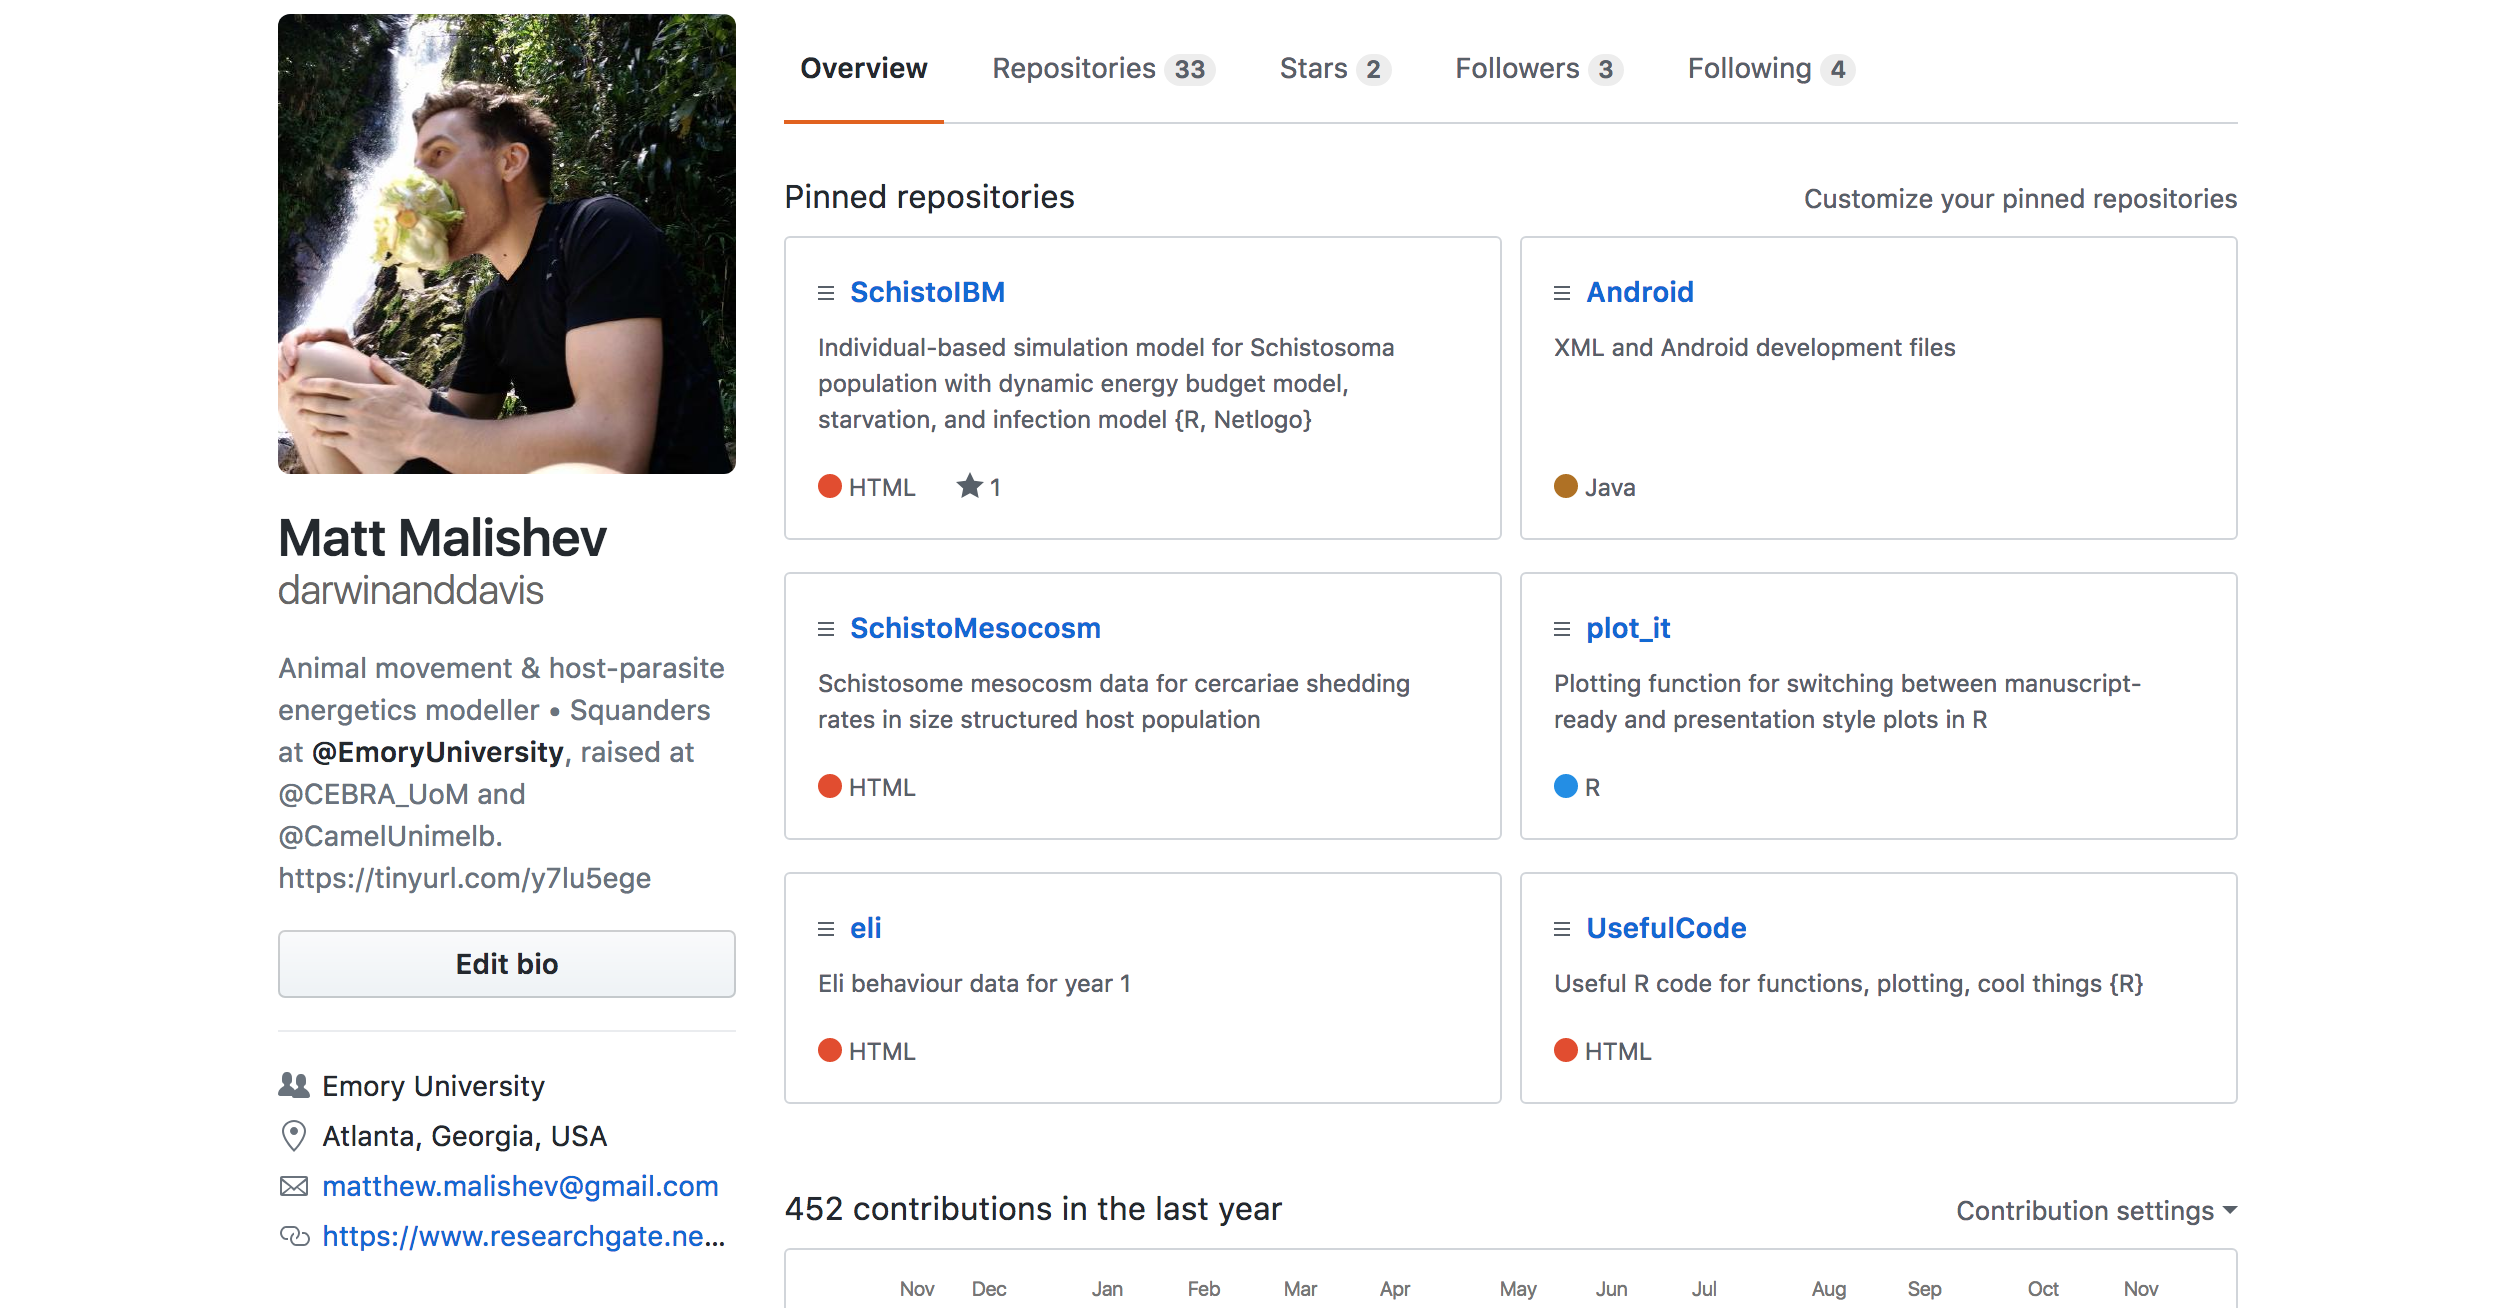
\includegraphics{loadingpage.png}
\caption{Github loading page}
\end{figure}

\begin{figure}
\centering
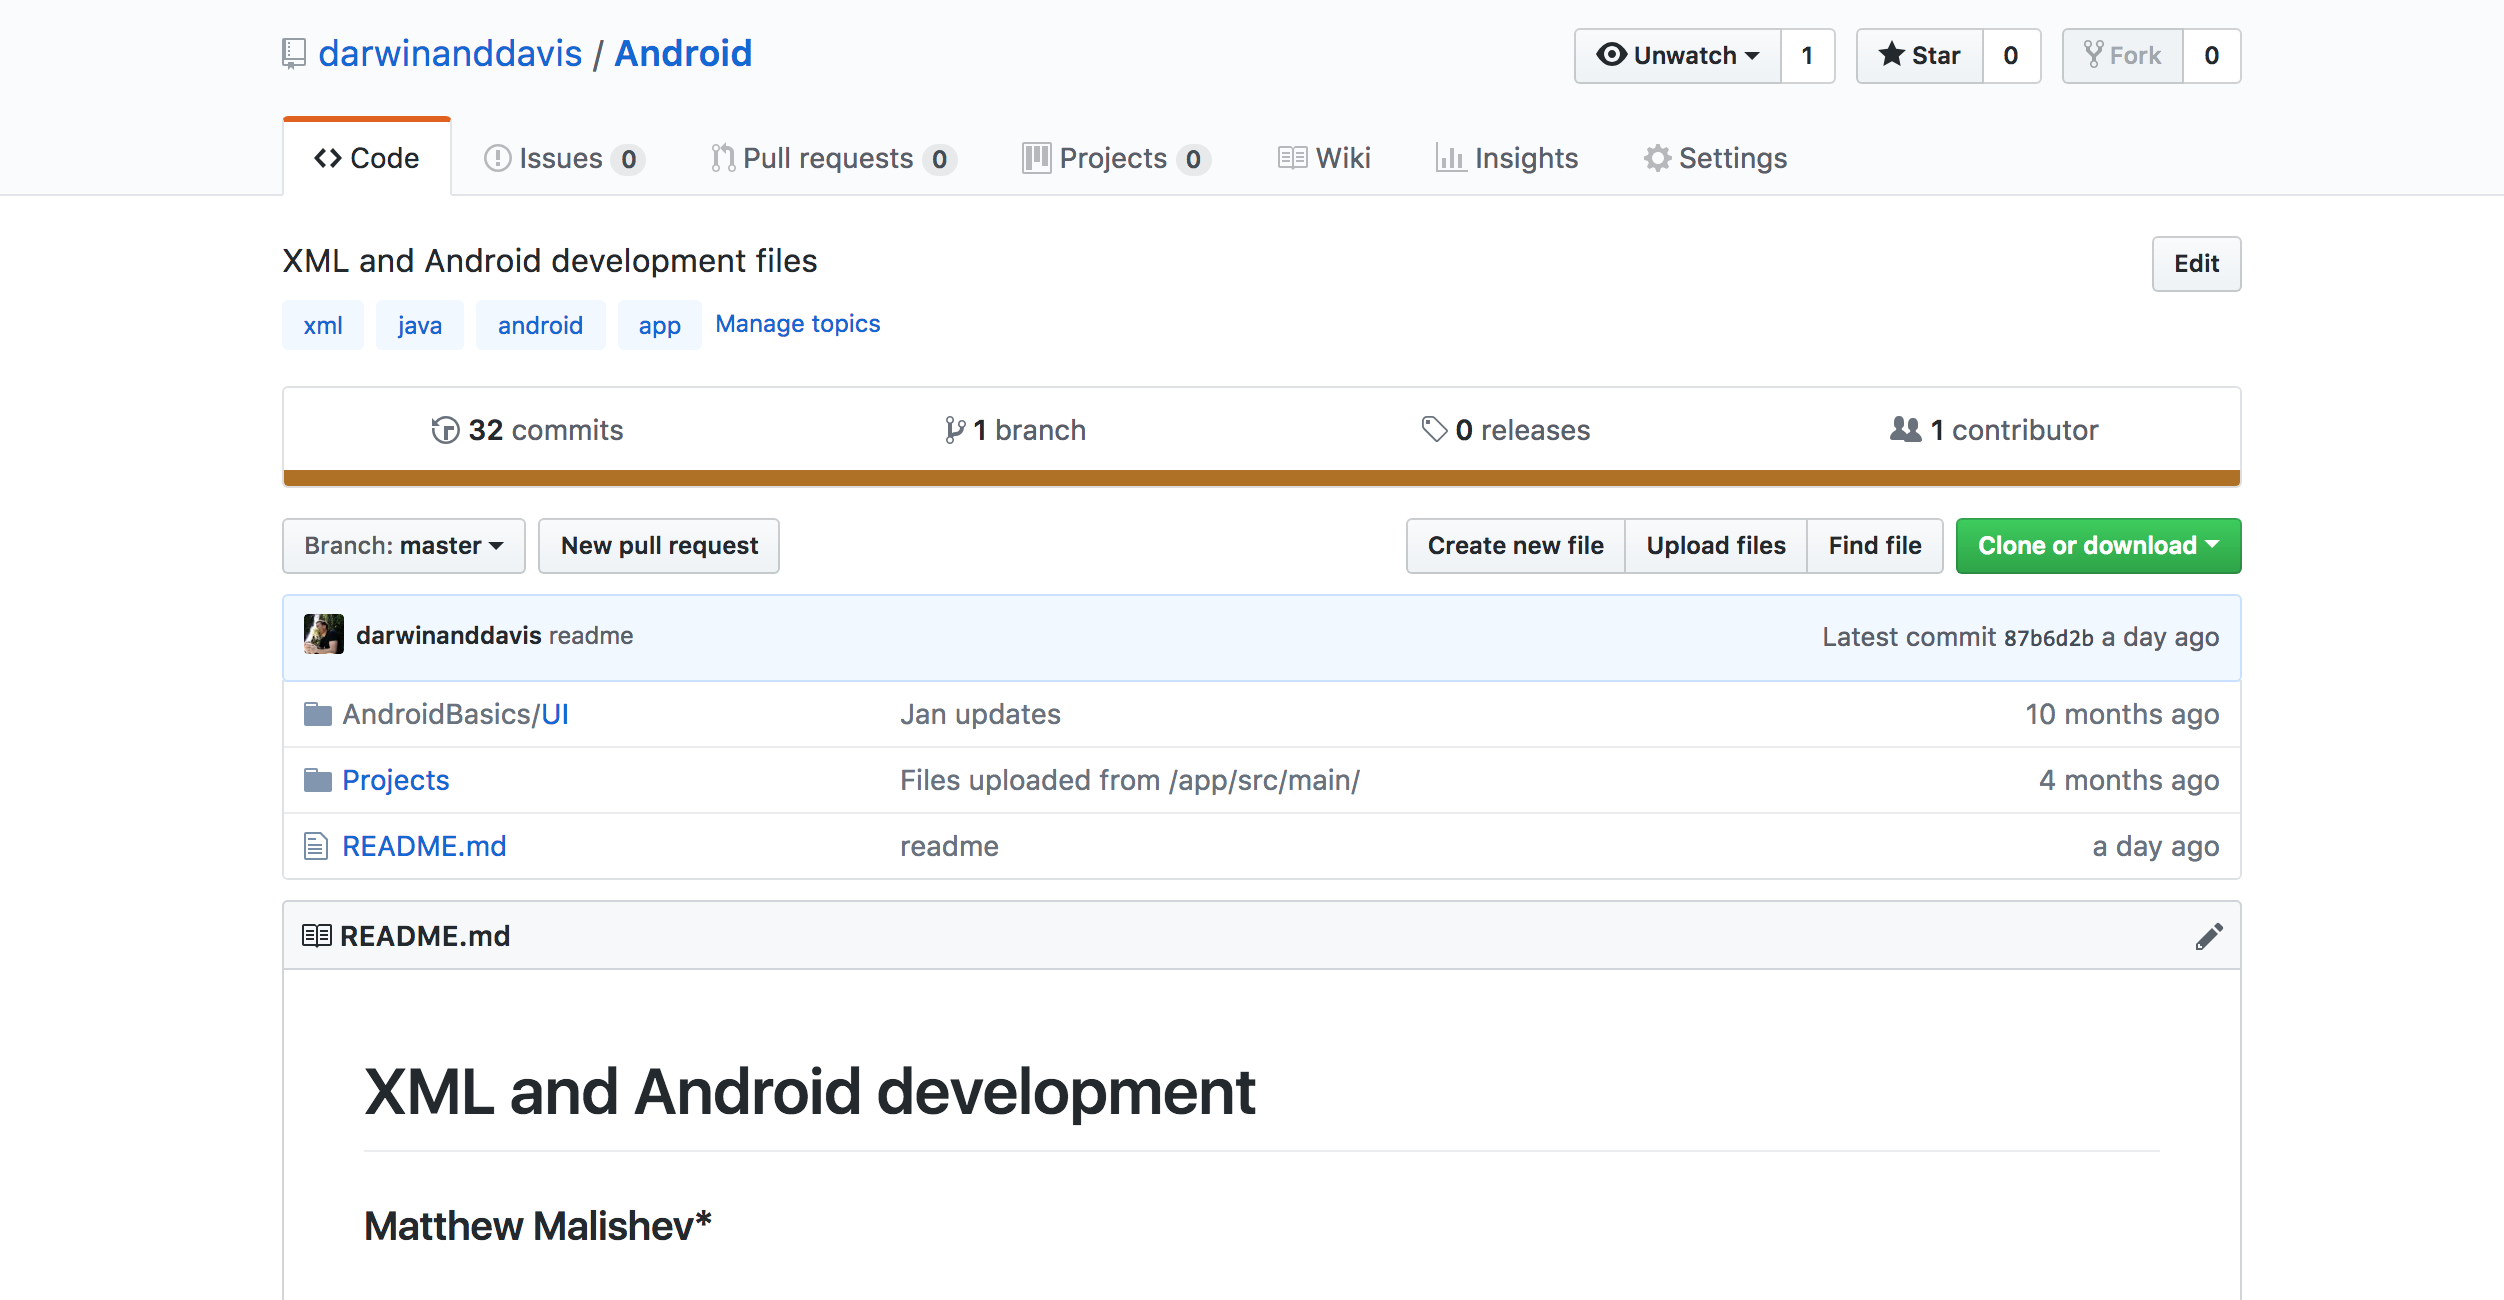
\includegraphics{repopage.png}
\caption{Repository loading page}
\end{figure}

\begin{figure}
\centering
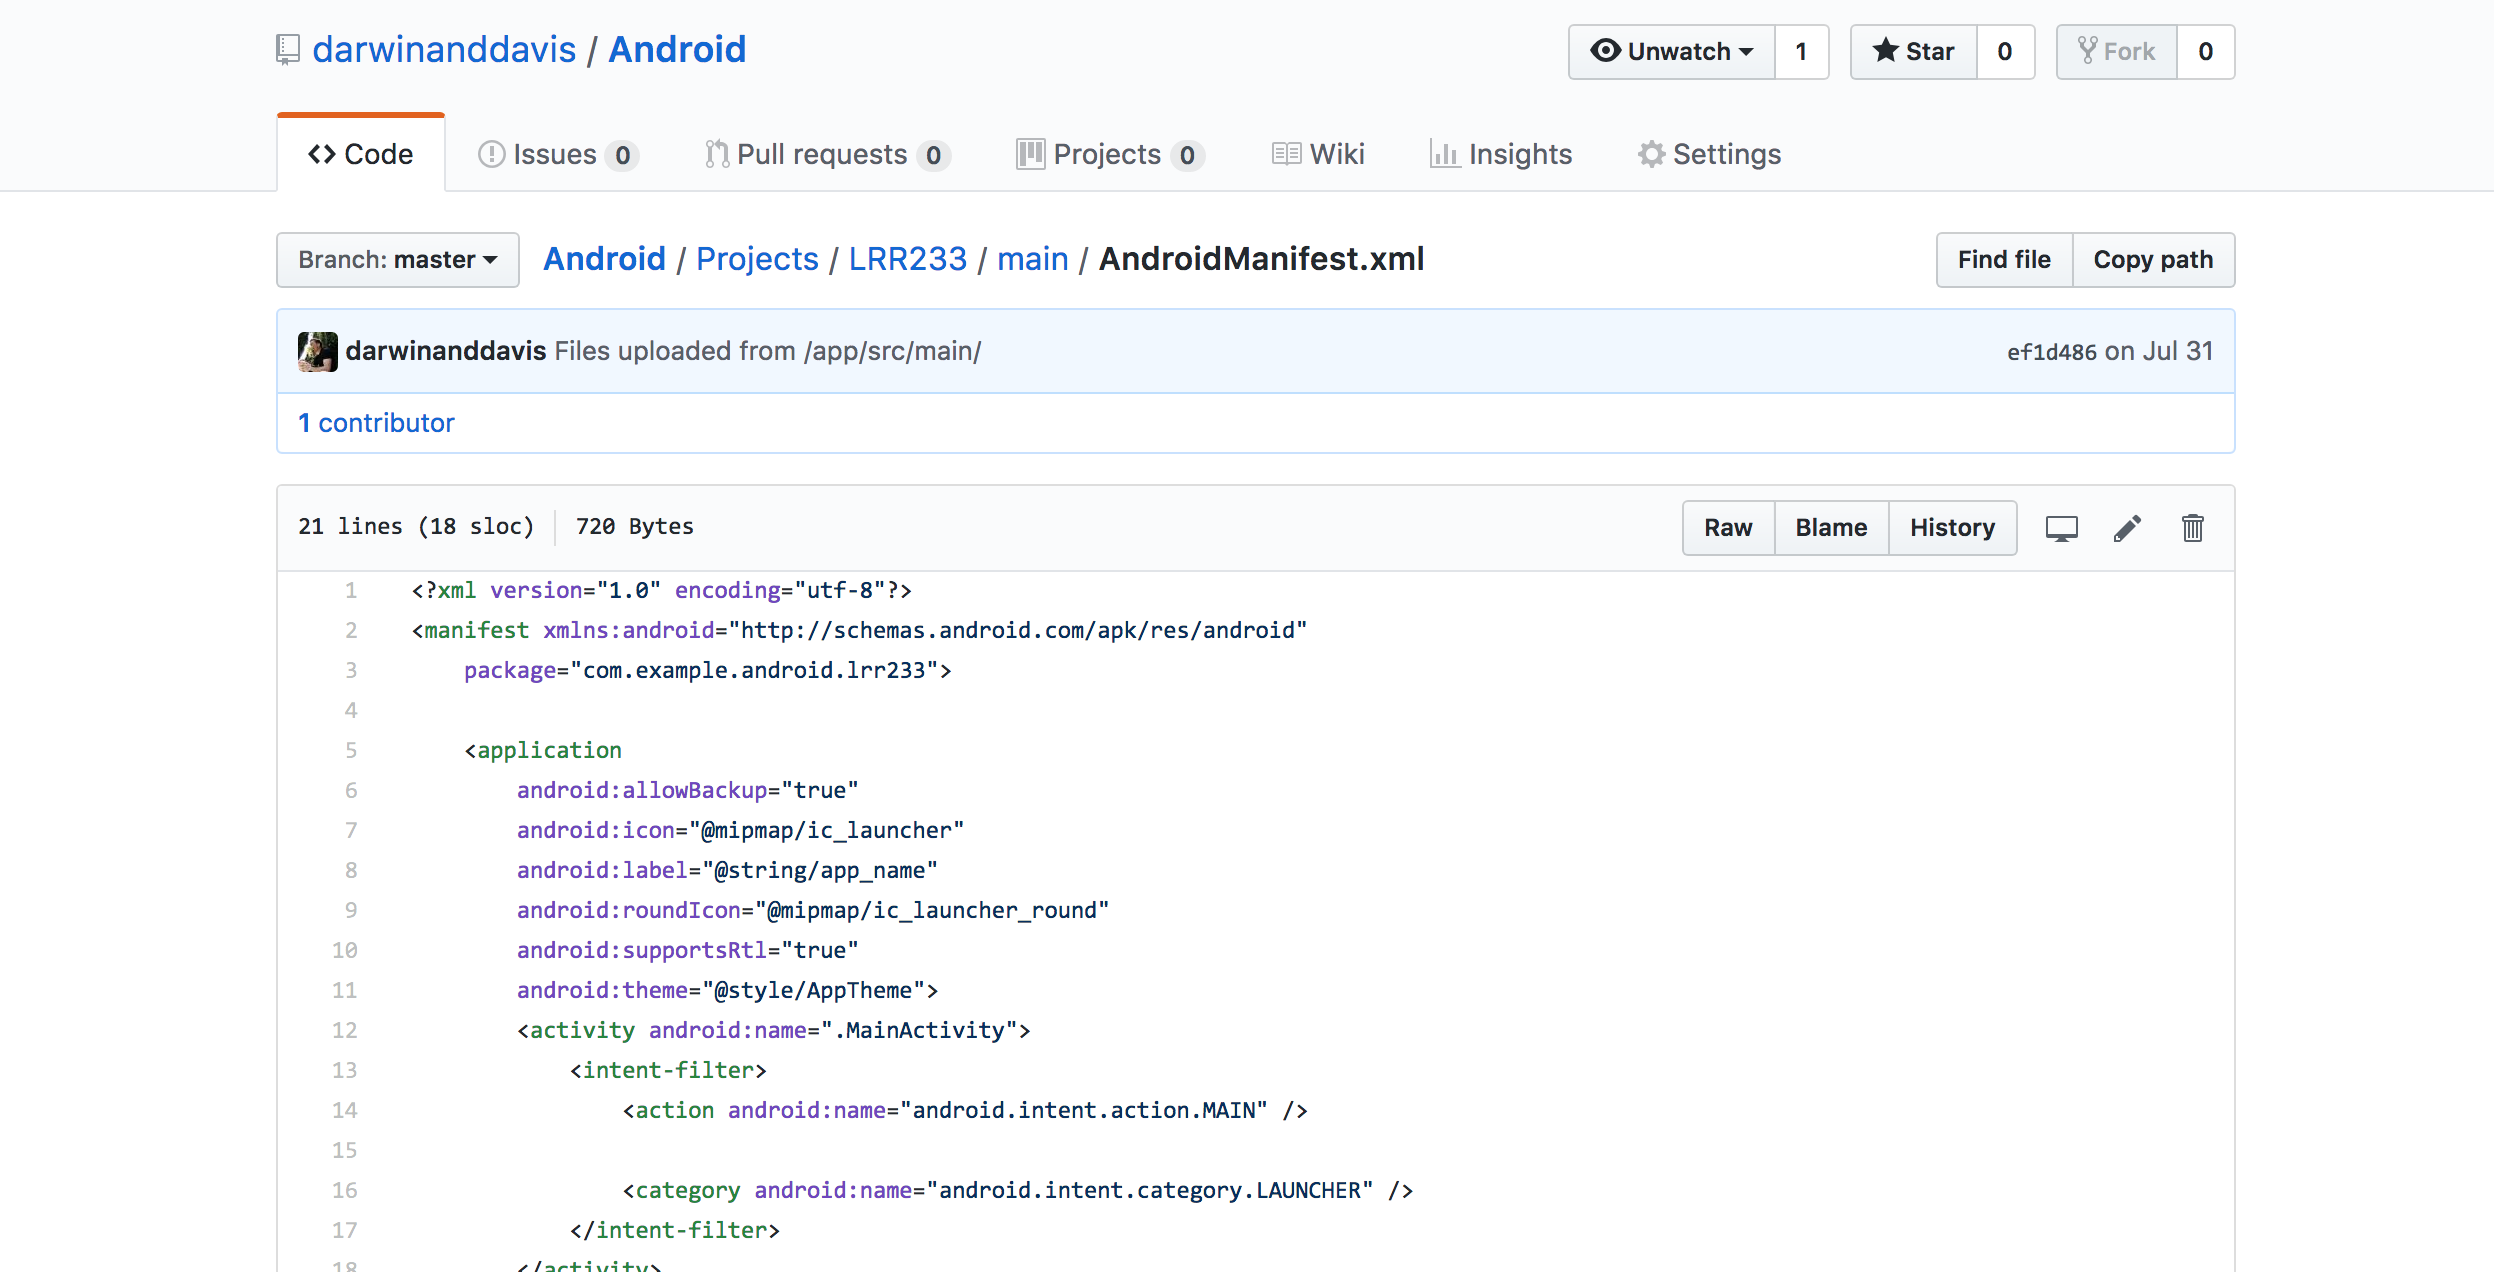
\includegraphics{filepage.png}
\caption{Inside of a file in a repository}
\end{figure}

\begin{figure}
\centering
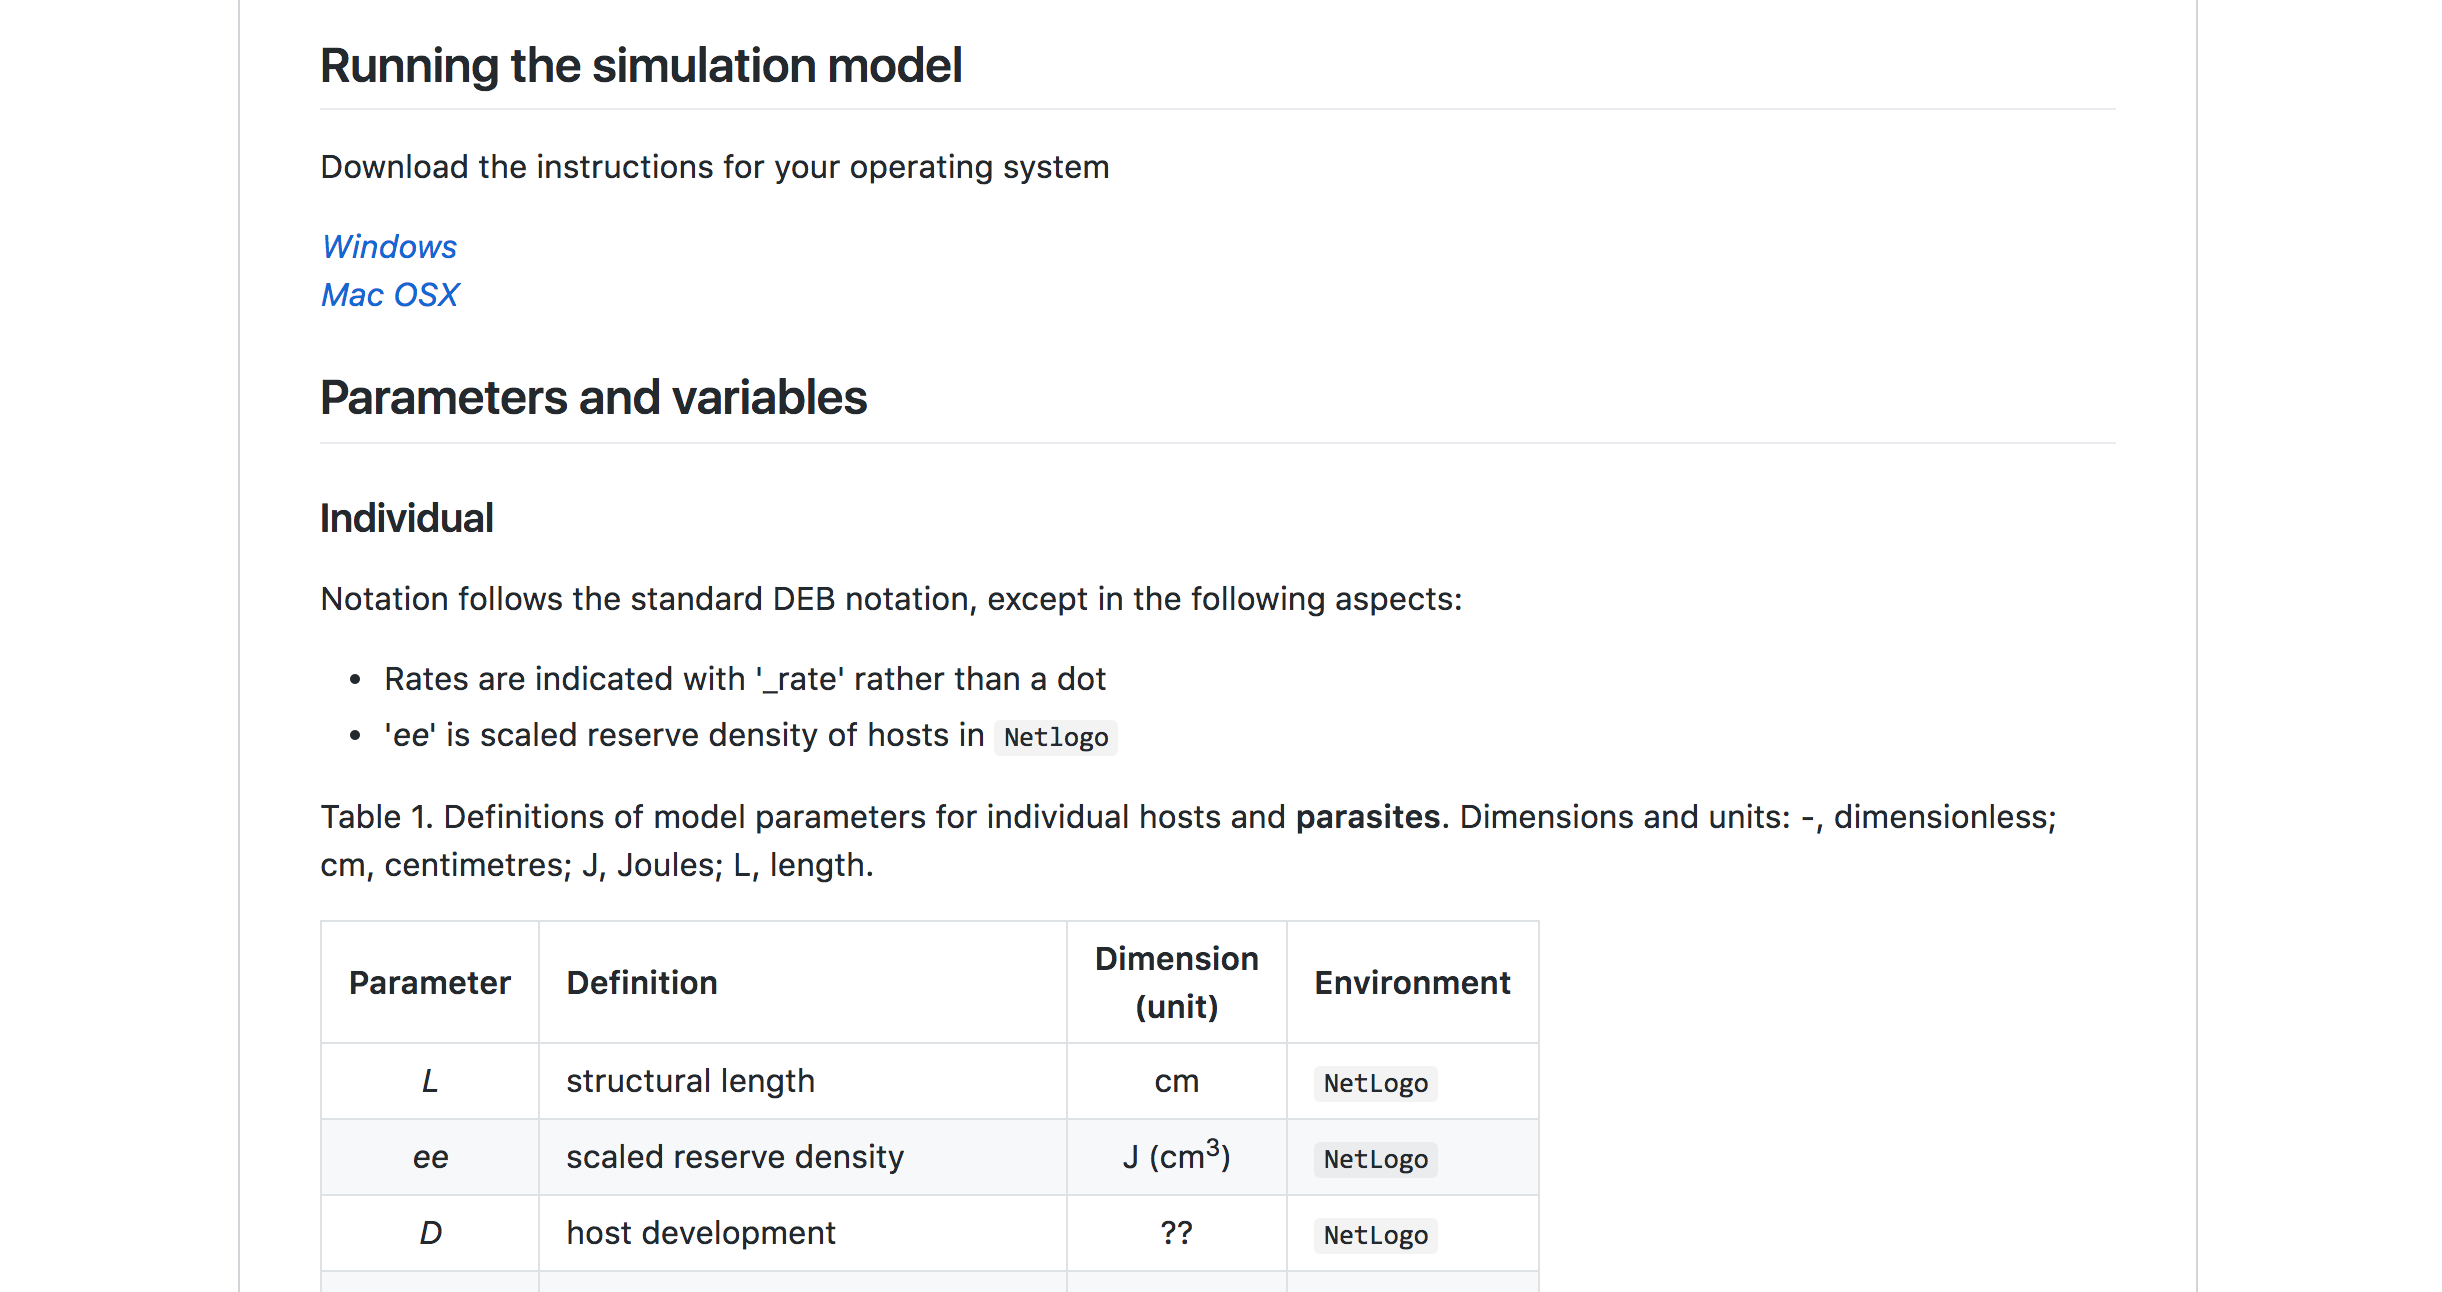
\includegraphics{readme.png}
\caption{Example of a README file}
\end{figure}

\newpage     

\subsection{Resources and references}\label{resources-and-references}

This section contains useful syntax and references for using git. We'll
be using the command line to talk with git.

\begin{itemize}
\tightlist
\item
  In Mac, this is found in \emph{Applications \textgreater{} Utilities
  \textgreater{} Terminal}.\\
\item
  In Windows, open the \textbf{Git Bash} application.
\end{itemize}

\subsubsection{\texorpdfstring{Commmon \texttt{git}
syntax}{Commmon git syntax}}\label{commmon-git-syntax}

\textbf{Note: commands require spaces between terms.}

Common \texttt{git} phrases

\emph{init} = initialise your git\\
\emph{push} = push your changes to a remote repository\\
\emph{pull} = pull changes made remotely to match local git changes\\
\emph{fetch} = re-align git changes from origin (remote) to master
(local) branch

Configure your credentials

\begin{Shaded}
\begin{Highlighting}[]
\FunctionTok{git}\NormalTok{ config --global user.name }\StringTok{"<your name>"}
\FunctionTok{git}\NormalTok{ config --global user.email }\StringTok{"<your email>"}  
\end{Highlighting}
\end{Shaded}

initialise a new git (local)

\begin{Shaded}
\begin{Highlighting}[]
\FunctionTok{git}\NormalTok{ init  }
\end{Highlighting}
\end{Shaded}

add all files in directory to git (local)

\begin{Shaded}
\begin{Highlighting}[]
\FunctionTok{git}\NormalTok{ add .}
\end{Highlighting}
\end{Shaded}

add individual file (local)

\begin{Shaded}
\begin{Highlighting}[]
\FunctionTok{git}\NormalTok{ add abstract.txt}
\end{Highlighting}
\end{Shaded}

check git activity (local)

\begin{Shaded}
\begin{Highlighting}[]
\FunctionTok{git}\NormalTok{ status }
\end{Highlighting}
\end{Shaded}

add remote origin source to push git (remote)

\begin{Shaded}
\begin{Highlighting}[]
\CommentTok{# two options  }
\ExtensionTok{get}\NormalTok{ remote set-url origin https://github.com/darwinanddavis/newtest.git  }
\FunctionTok{git}\NormalTok{ remote add origin https://github.com/darwinanddavis/newtest.git}
\end{Highlighting}
\end{Shaded}

push git changes to origin (your remote location) from your master
(local) branch

\begin{Shaded}
\begin{Highlighting}[]
\FunctionTok{git}\NormalTok{ push origin master }
\end{Highlighting}
\end{Shaded}

check latest git activity (local)

\begin{Shaded}
\begin{Highlighting}[]
\FunctionTok{git}\NormalTok{ log}
\end{Highlighting}
\end{Shaded}

check what remote locations you have available to push your gits

\begin{Shaded}
\begin{Highlighting}[]
\FunctionTok{git}\NormalTok{ remote -v }\CommentTok{# v = verbose    }
\end{Highlighting}
\end{Shaded}

add another remote destination (on github) called `github' (remote) and
push your staged git (file changes) to that remote location from your
master (local) branch

\begin{Shaded}
\begin{Highlighting}[]
\FunctionTok{git}\NormalTok{ remote add github https://github.com/darwinanddavis/newtest.git }
\FunctionTok{git}\NormalTok{ push github master }
\end{Highlighting}
\end{Shaded}

See these references for a brief intro to using the command line in
\href{https://macpaw.com/how-to/use-terminal-on-mac}{Mac} and
\href{https://www.computerhope.com/issues/chusedos.htm}{Windows}.

~

\subsubsection{Useful command line
syntax}\label{useful-command-line-syntax}

\textbf{Note: commands require spaces between terms.}

\texttt{cd\ \textasciitilde{}/Documents} change working dir to
`Documents'. \texttt{cd\ ..} move one level up

\texttt{pwd} print current working dir

\texttt{ls} list files in working dir

\texttt{mkdir\ newfolder} make new working dir

\texttt{touch\ text.txt} create new file (called text.txt)

\subsubsection{More useful syntax}\label{more-useful-syntax}

\textbf{Note: commands require spaces between terms.}

copy files from \emph{source} to \emph{destination}. e.g.~cp
/Users/mydir/README.txt \textasciitilde{}/Documents\\
\texttt{cp\ source\ destination}

copy all folders, subfolders, and files from \emph{source} to
\emph{destination}\\
\texttt{cp\ -R\ source\ destination}

move files or folders from \emph{source} to \emph{destination} (no need
for \texttt{-R})\\
\texttt{mv\ source\ destination}

move multiple files with the * wildcard, which copies all .rtf files.
The tilde (\textasciitilde{}) symbol is a shortcut for your Home folder,
which contains `/Desktop'.\\
\texttt{cp\ \textasciitilde{}/Desktop/*.rtf\ \textasciitilde{}/Documents}

rename files\\
\texttt{mv\ \textasciitilde{}/Desktop/MyFile.rtf\ \textasciitilde{}/Desktop/MyFile-old.rtf}\\
\texttt{cp\ \textasciitilde{}/Desktop/MyFile.rtf\ \textasciitilde{}/Documents/MyFile-old.rtf}

\subsubsection{Example of command line
workflow}\label{example-of-command-line-workflow}

Open \emph{Terminal/cmd}

\begin{Shaded}
\begin{Highlighting}[]
\BuiltInTok{cd}\NormalTok{ ~/Documents/ }\CommentTok{# change working dir}
\FunctionTok{ls} \CommentTok{# list dir contents      }
\end{Highlighting}
\end{Shaded}

Open \emph{Finder/Windows}. Make a new project on your local comp.

\begin{Shaded}
\begin{Highlighting}[]
\CommentTok{# create new project  }
\CommentTok{### <b> }
\BuiltInTok{cd}\NormalTok{ ~/Documents}
\CommentTok{### </b>}
\CommentTok{# create new file }
\CommentTok{### <b> }
\FunctionTok{touch}\NormalTok{ test.txt  }
\ExtensionTok{open}\NormalTok{ test.txt  }
\CommentTok{### </b> }
\CommentTok{# make a new folder  }
\CommentTok{### <b> }
\FunctionTok{mkdir}\NormalTok{ newgit  }
\CommentTok{### </b>}
\CommentTok{# navigate to that folder  }
\CommentTok{### <b>}
\BuiltInTok{cd}\NormalTok{ newgit}
\FunctionTok{ls}\NormalTok{ -a  }
\CommentTok{### </b>   }
\end{Highlighting}
\end{Shaded}

Create a new file in the command line

\begin{Shaded}
\begin{Highlighting}[]
\CommentTok{# navigate to your new git repo  }
\CommentTok{### <b>}
\BuiltInTok{pwd}  
\BuiltInTok{cd}\NormalTok{ ~/Documents/newgit}
\CommentTok{### </b> }

\CommentTok{# move the new file into the git repo      }
\CommentTok{### <b> }
\FunctionTok{mv}\NormalTok{ ~/Documents/test.txt ~/Documents/newgit}
\FunctionTok{ls}  
\CommentTok{### </b> }
\end{Highlighting}
\end{Shaded}

\subsection{References}\label{references}

\href{https://git-scm.com/book/en/v2/Getting-Started-Installing-Git}{Installing
git}

\href{https://github.com/}{Sign up to Github}

\href{https://git-scm.com/book/en/v2/Getting-Started-About-Version-Control}{Version
control with git}

\href{https://macpaw.com/how-to/use-terminal-on-mac}{Terminal in Mac}

\href{https://www.computerhope.com/issues/chusedos.htm}{Command line in
Windows}

\href{}{}

\subsection{Maintainer}\label{maintainer}

Matt Malishev\\
\href{https://github.com/darwinanddavis}{Github} \textbar{}
\href{https://www.researchgate.net/profile/Matt_Malishev}{Website}\\
matthew.malishev {[}at{]} emory.edu

\printbibliography

\end{document}
